\chapter{Simulation}
\label{sim}
Circuit simulation uses mathematical models to replicate the behaviour of an actual device or circuit. Simulation software allows for modeling of circuit operation. Simulating a circuit's behaviour before actually building it can greatly improve design efficiency by making faulty designs known as such, and providing insight into the behavior of electronics circuit designs. Oscad uses Ngspice for mixed-level/mixed-signal circuit simulation. 
\section{Analysis}
Oscad supports three types of analyses which are depicted below:
\begin{enumerate}
\item DC Analysis (Operating Point and DC Sweep) 
\item AC Small-Signal Analysis 
\item Transient Analysis 
\end{enumerate}
In order to understand the relationship between the different analyses and the two underlying simulation algorithms of ngspice, it is important to understand what is meant by each analysis type. This is detailed below. 
\subsection{DC Analysis}
The dc analysis portion of ngspice determines the dc operating point of the circuit with inductors shorted and capacitors opened. The dc analysis options are specified on the .DC, .TF, and .OP control lines. 
There is assumed to be no time dependence on any of the sources within the system description. The simulator algorithm subdivides the circuit into those portions which require the analog simulator algorithm and those which require the event-driven algorithm. Each subsystem block is then iterated to solution, with the interfaces between analog nodes and event-driven nodes iterated for consistency across the entire system. 

Once stable values are obtained for all nodes in the system, the analysis halts and the results may be displayed or printed out as you request them.
 
A dc analysis is automatically performed prior to a transient analysis to determine the transient initial conditions, and prior to an ac small-signal analysis to determine the linearized, small- signal models for nonlinear devices. If requested, the dc small-signal value of a transfer function (ratio of output variable to input source), input resistance, and output resistance is also computed as a part of the dc solution. The dc analysis can also be used to generate dc transfer curves: a specified independent voltage, current source, resistor or temperature1 is stepped over a user- specified range and the dc output variables are stored for each sequential source value. 
\subsection{AC Small-signal Analysis}
AC analysis is limited to analog nodes and represents the small signal, sinusoidal solution of the analog system described at a particular frequency or set of frequencies. This analysis is similar to the DC analysis in that it represents the steady-state behavior of the described system with a single input node at a given set of stimulus frequencies. 

The program first computes the dc operating point of the circuit and determines linearized, small-signal models for all of the nonlinear devices in the circuit. The resultant linear circuit is then analyzed over a user-specified range of frequencies. The desired output of an ac small-signal analysis is usually a transfer function (voltage gain, transimpedance, etc). If the circuit has only one ac input, it is convenient to set that input to unity and zero phase, so that output variables have the same value as the transfer function of the output variable with respect to the input.
\subsection{Transient Analysis}
Transient analysis is an extension of DC analysis to the time domain. A transient analysis be-gins by obtaining a DC solution to provide a point of departure for simulating time-varying behavior. Once the DC solution is obtained, the time-dependent aspects of the system are rein- troduced, and the two simulator algorithms incrementally solve for the time varying behavior of the entire system. Inconsistencies in node values are resolved by the two simulation algorithms such that the time-dependent waveforms created by the analysis are consistent across the entire simulated time interval. Resulting time-varying descriptions of node behavior for the specified time interval are accessible to you. All sources which are not time dependent (for example, power supplies) are set to their dc value. The transient time interval is specified on a .TRAN control line. 
\section{Analysis Inserter}
\label{ana}
In order to simulate a circuit, an user must define the type of simulation to be run. The type of analysis includes Operating point analysis, DC analysis, AC analysis, transient analysis etc. Also, user needs to specify the option corresponding to the analysis. Analysis inserter generate the command for ngspice. When you click on analysis inserter the window shown in Figure \ref{1} will appear. It consists of type of analysis in top, and details which are needed to sweep the input value. 
\begin{figure}
\centering
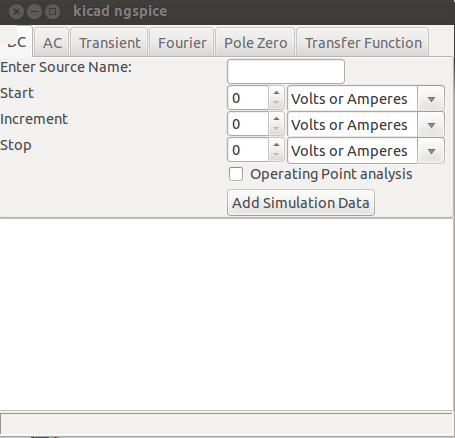
\includegraphics[width=\textwidth]{figures/1}
\caption{Analysis inserter GUI}
\label{1}
\end{figure}
\subsection{DC Analysis}
By default DC analysis window will open when you click on analysis inserter, where we need to give the details of  input source name, start point of input, increment and  stop point. When you click on “Add Simulation Data” the window shown in Figure \ref{2} will appear.
\begin{figure}
\centering
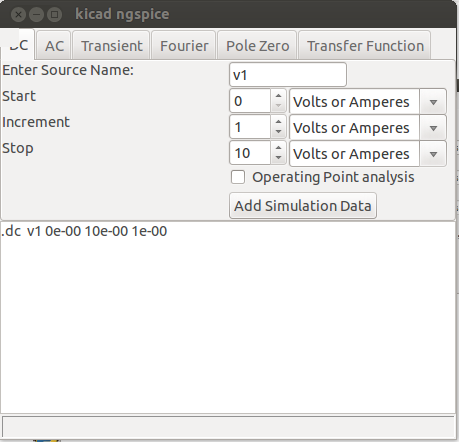
\includegraphics[width=\textwidth]{figures/2}
\caption{DC Analysis}
\label{2}
\end{figure}
In this example we consider 'v1' as a input voltage source which starts from '0Volt' and incremented by '1Volt' and stopped at '10Volt'. The syntax generated by this process is of the form

\textit{. dc sourcename vstart vstop vincr}

The .dc line defines the dc transfer curve source and sweep limits (again with capacitors open and inductors shorted). srcnam is the name of an independent voltage or current source, a resistor or the circuit temperature. vstart, vstop, and vincr are the starting, final, and incrementing values respectively. 

When we select “.op” option then the window given in Figure \ref{3} will appear.
\begin{figure}
\centering
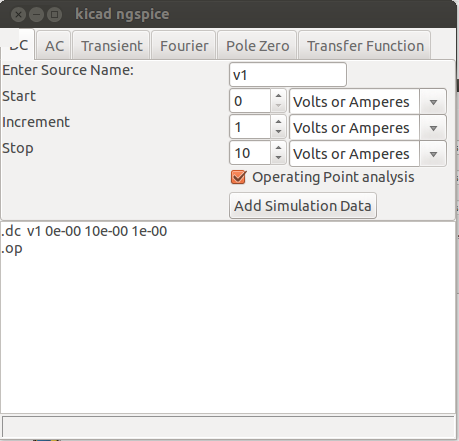
\includegraphics[width=\textwidth]{figures/3}
\caption{OP Analysis}
\label{3}
\end{figure}
{\tt .op } - The inclusion of this line in an input file directs ngspice to determine the dc operating point of the circuit with inductors shorted and capacitors opened. 
\subsection{AC Analysis}
When you click on “AC” the window given in Figure \ref{4} will appear.
\begin{figure}
\centering
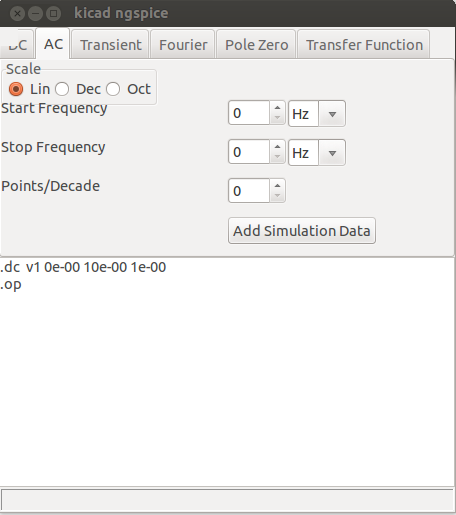
\includegraphics[width=\textwidth]{figures/4}
\caption{AC Analysis GUI}
\label{4}
\end{figure}
This window will ask you to enter the detail of “scale”, “start frequency”, “stop frequency”, “numbers of point”.

After entering all these values and clicking on “Add Simulation Data” you will get the window as shown in Figure \ref{5}.
\begin{figure}
\centering
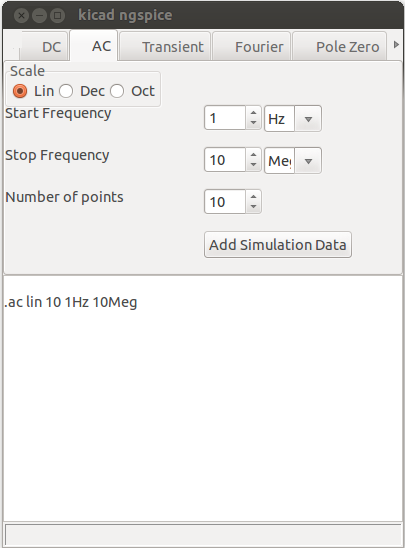
\includegraphics[width=\textwidth]{figures/5}
\caption{AC Analysis example}
\label{5}
\end{figure}
This window shows that start frequency is “1 Hz”, stop frequency is “10 MegHz” and  numbers of point “10”.
The syntax generated by this is of the form: 

{\tt .ac dec nd fstart fstop }\\
{\tt .ac oct no fstart fstop }\\
{\tt .ac lin np fstart fstop }

{\tt dec} stands for decade variation, and {\tt nd} is the number of points per decade. {\tt oct} stands for octave variation, and {\tt no} is the number of points per octave. {\tt lin} stands for linear variation, and np is the number of points. {\tt fstart} is the starting frequency, and {\tt fstop} is the final frequency. If this line is included in the input file, ngspice performs an AC analysis of the circuit over the specified frequency range. Note that in order for this analysis to be meaningful, at least one independent source must have been specified with an ac value.
\subsection{Transient Analysis}
If you click on the option `Transient', the window given in Figure \ref{6} will appear.
\begin{figure}
\centering
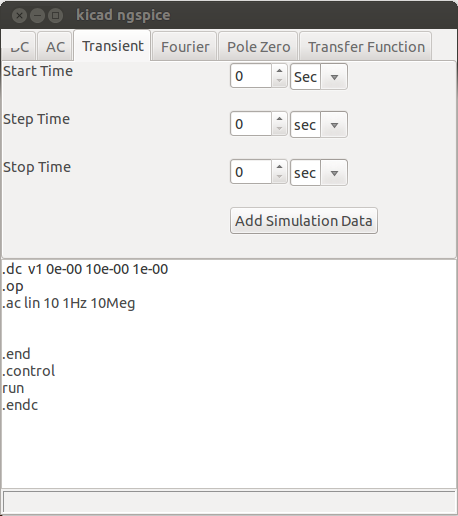
\includegraphics[width=\textwidth]{figures/6}
\caption{Transient Analysis - GUI}
\label{6}
\end{figure}
Above window will ask to enter the details like “start time”, “step time”, “stop time”
After entering these values when you click on “Add Simulation Data” you will get the window as shown in Figure \ref{7}.
\begin{figure}
\centering
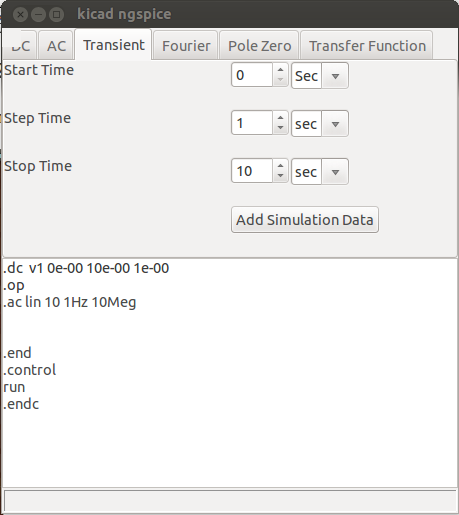
\includegraphics[width=\textwidth]{figures/7}
\caption{Transient Analysis - example}
\label{7}
\end{figure}
Above window shows that start time is “0 sec”, step time is “1 sec” and stop time is “10 sec”.
The syntax generated by this process is of the form:

{\tt .tran tstep tstop <tstart <tmax >>  <uic>}

tstep is the printing or plotting increment for line-printer output. For use with the postprocessor, tstep is the suggested computing increment. tstop is the final time, and tstart is the initial time. If tstart is omitted, it is assumed to be zero. The transient analysis always begins at time zero. In the interval <zero, tstart>, the circuit is analyzed (to reach a steady state), but no outputs are stored. In the interval <tstart, tstop>, the circuit is analyzed and outputs are stored. tmax is the maximum stepsize that ngspice uses; for default, the program chooses either tstep or (tstop-tstart)/50.0, whichever is smaller. tmax is useful when one wishes to guarantee a computing interval which is smaller than the printer increment, tstep. An initial transient operating point at time zero is calculated according to the following procedure: all independent voltages and currents are applied with their time zero values, all capacitances are opened, inductances are shorted, the non linear device equations are solved iteratively. uic (use initial conditions) is an optional keyword which indicates that the user does not want ngspice to solve for the quiescent operating point before beginning the transient analysis. 

After entering the details of analysis we need to save the analysis file. These details will be store in “analysis” file. Use following process to save the analysis file.
Move your cursor to “file” as shown in figure \ref{8} then click on it. “save” option will come after clicking on file. Click on save. The file will be saved in analysis file.
\begin{figure}
\centering
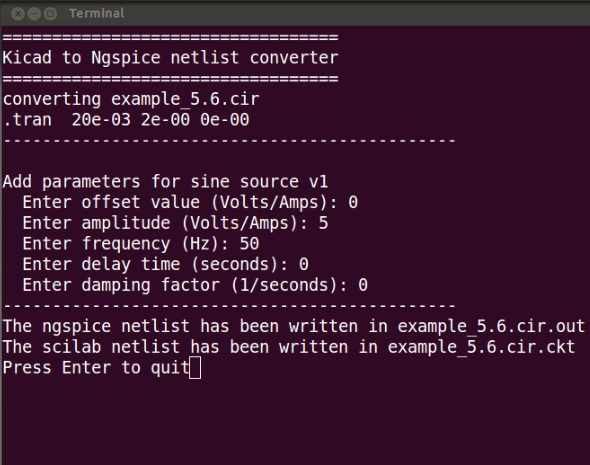
\includegraphics[width=\textwidth]{figures/8}
\caption{Saving the analysis information to netlist}
\label{8}
\end{figure}
\section{KiCad to Ngspice Conversion}
A schematic editor provides a netlist file, which describes the electrical connections between circuit components. Eeschema provides a SPICE netlist which can not be directly used for simulation due to compatibility issues. After Analysis insertion click on Kicad to Ngspice tool from the Oscad toolbar. Oscad netlist converter performs following operation to generate Ngspice compatible netlist.
\subsection{Insert parameters for fictitious components}
For simulation of the circuit, the value of sources must be specified, e.g., for sine wave voltage source, parameters (frequency, amplitude, offset etc.) are required to be 
entered. Our netlist converter scan the netlist file and ask for parameter values for the sources wherever required. 
When we click on kicad to ngspice converter, a terminal window appears. It asks for various parameter values. This varies depending upon the voltage/current sources added in the schematic for simulation.
\begin{enumerate}
\item When sinusoidal source is available in schematic
\begin{figure}
\centering
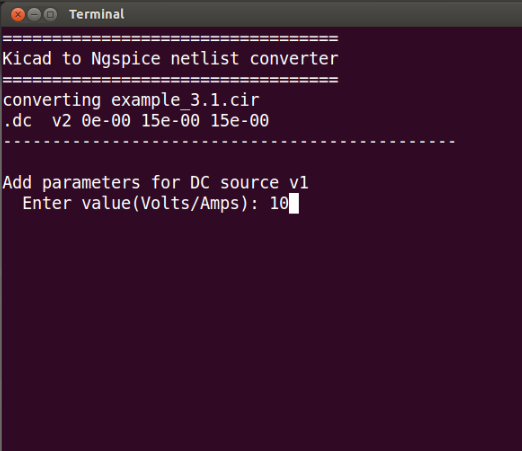
\includegraphics[width=\textwidth]{figures/9}
\caption{Parameters to be added for sinusoidal source}
\label{9}
\end{figure}
- in this terminal we will add all the details of sinusoidal source like “offset value”, “amplitude”, “frequency”, delay time”, “damping factor”.
\item When DC source of unknown value is available in schematic
\begin{figure}
\centering
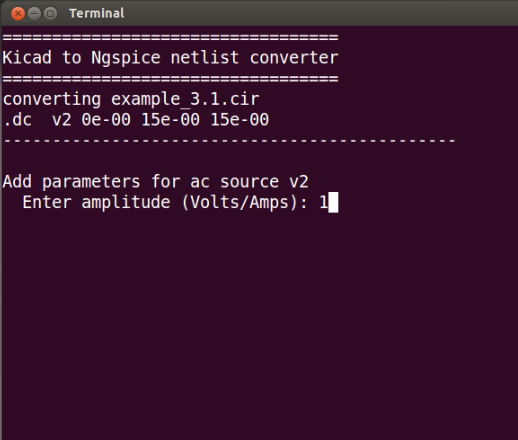
\includegraphics[width=\textwidth]{figures/10}
\caption{Parameters to be added for dc source}
\label{10}
\end{figure}
- It will ask for the value of DC source, in our case value of DC is 10V.
\item When AC source is available in schematic
\begin{figure}
\centering
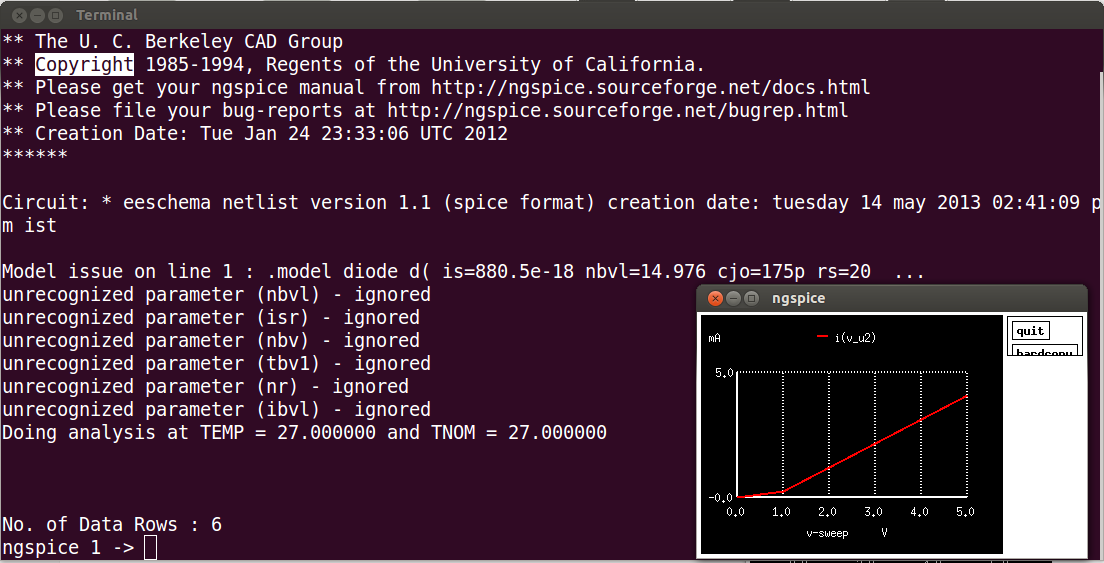
\includegraphics[width=\textwidth]{figures/11}
\caption{Parameters to be added for ac source}
\label{11}
\end{figure}
- It will ask for amplitude of AC, in our case value is 1V.
\end{enumerate}
\subsection{Convert IC into discrete blocks}
As Eeschema is intended for PCB Designing, it gives netlist in terms of IC not components, e.g., if design contains a two-input Nand gate, then in the netlist, IC 7400 appears instead of the Nand gate. OSCAD netlist converter converts the IC into discrete blocks with considering proper input and output connections and IC specifications (voltage levels, speed of the operation etc.). 
\subsection{Insert Digital-to-Analog (D-to-A) and Analog-to-Digital (A-to-D) converter at appropriate places}
Oscad provides capability to perform mix mode simulation. Thus circuits with analog and digital components can be analyzed. In order to simulate such kind of circuits, D-to-A and A-to-D converter are inserted at appropriate places. We assume the netlist generated from Eeschema has analog connections and for digital components, we have added A-to-D converter for inputs and D-to-A converter for outputs.
\subsection{Insert plotting and printing statements}
There is a library for plotting and printing the circuit solution (voltages and currents). The netlist converter adds appropriate printing and plotting commands (current or voltage plot, or single or differential plot) in the netlist depending on the print/plot components. Ngspice is able to find the current through voltage sources only. Netlist converter inserts a zero volt voltage source in series with the component through which current needs to be computed. 
\subsection{Insert analysis and option}
Oscad netlist converter inserts analysis information created in Section \ref{ana} into the netlist.
\subsection{Insert models and sub-circuits}
Oscad netlist converter inserts models or sub-circuits for required components into the netlist. 
\section{Simulation}
After Kicad to Ngspice we get {\tt .cir.out} file which is compatible to Ngpice simulation software.
\subsection{Ngspice}
Ngspice is a general-purpose circuit simulation program for nonlinear and linear analyses. Circuits may contain resistors, capacitors, inductors, mutual inductors, independent or dependent voltage and current sources, loss-less and lossy transmission lines, switches, uniform distributed RC lines, and the five most common semiconductor devices: diodes, BJTs, JFETs, MESFETs, and MOSFETs. 

Ngspice is an update of Spice3f5, the last Berkeley’s release of Spice3 simulator family. Ngspice is being developed to include new features to existing Spice3f5 and to fix its bugs. Improving a complex software like a circuit simulator is a very hard task and, while some improvements have been made, most of the work has been done on bug fixing and code refactoring. 

Ngspice supports mixed-signal simulation through the integration of XSPICE code into it. XSPICE software, developed as an extension to Spice3C1 from GeorgiaTech, has been ported to ngspice to provide “board” level and mixed-signal simulation.
\subsection{Ngspice simulation in Oscad}
After clicking on Ngspice from the Oscad toolbar, we will get Ngspice terminal and waveform window as shown in Figure \ref{12}.
\begin{figure}
\centering
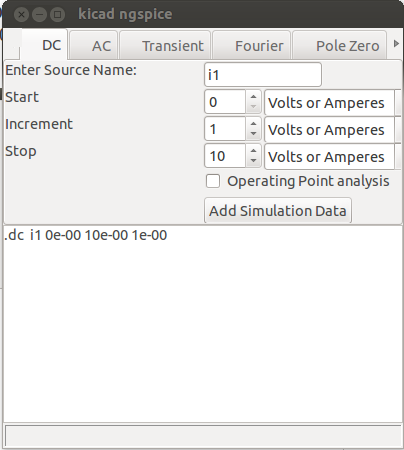
\includegraphics[width=\textwidth]{figures/12}
\caption{Ngspice simulation of {\tt .cir.out} file}
\label{12}
\end{figure}
\section{Simulation Examples}
\subsection{DC simulation example}
\label{dc}
Consider the nodal analysis example giving in the Examples available in the OScad webpage {\tt www.oscad.net}.  we  open Kicad and generate spice netlist as given in section (schematic chapter), we click on “analysis inserter”,Here we decide which type of analysis we want to do.

{\tt DC Analysis} -  We click on DC  and Enter the details “source name”=i1, “start”=0A, “Increment”=1A, “stop”=10A and then click on Add Simulation data as shown in Figure \ref{13}.
\begin{figure}
\centering
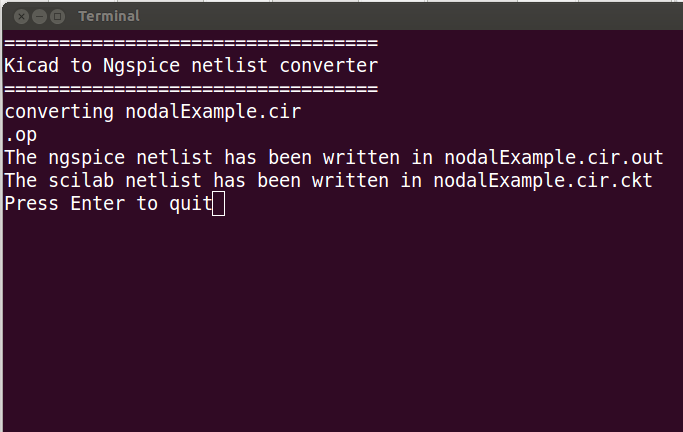
\includegraphics[width=\textwidth]{figures/13}
\caption{DC analysis - adding simulation data}
\label{12}
\end{figure}
Now we click on Kicad to Ngpice which will show the  terminal given in Figure \ref{14}. Press 'enter' key.
\begin{figure}
\centering
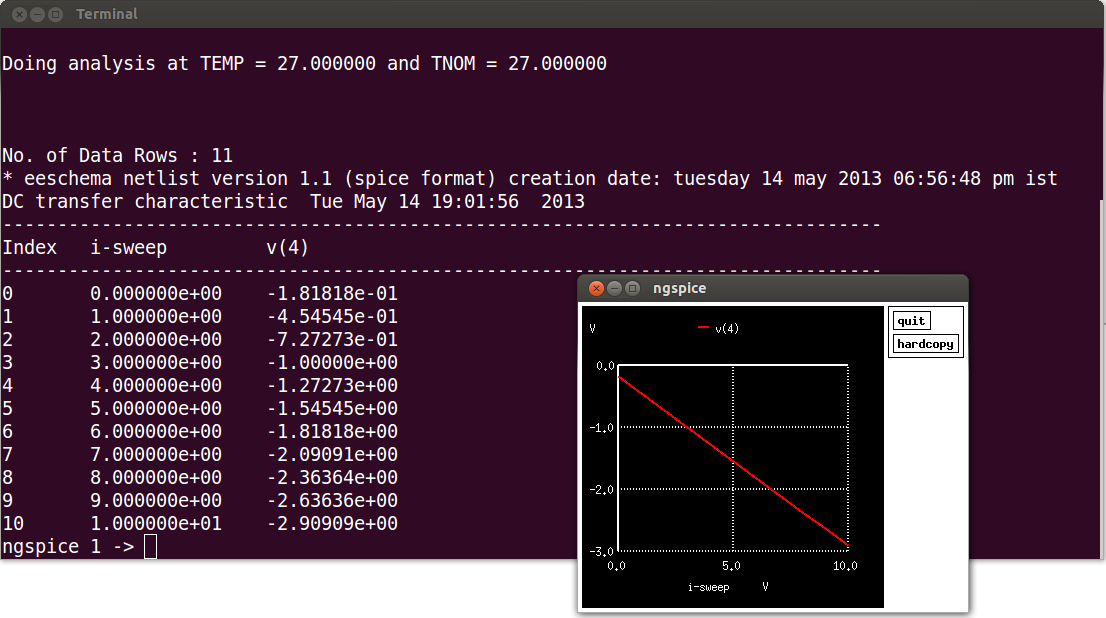
\includegraphics[width=\textwidth]{figures/14}
\caption{Terminal - KiCad to Ngspice netlist converter}
\label{14}
\end{figure}
After this we click on Ngspice button which will show Ngspice terminal with waveform window as shown in the Figure \ref{15}.
\begin{figure}
\centering
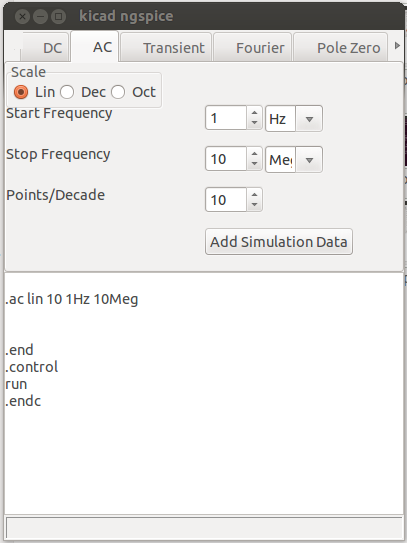
\includegraphics[width=\textwidth]{figures/15}
\caption{Ngspice simulation result}
\label{15}
\end{figure}
\subsection{Example of AC and Transient Analysis}
Consider the RC\_ac example folder from the Example folder available in Oscad website and follow the steps given in section \ref{dc}

{\tt AC Analysis} -  We click on AC and add details like “scale”, “start frequency”, “stop frequency”, “number of points” and then click on Add simulation data. This is shown in Figure \ref{16}.
\begin{figure}
\centering
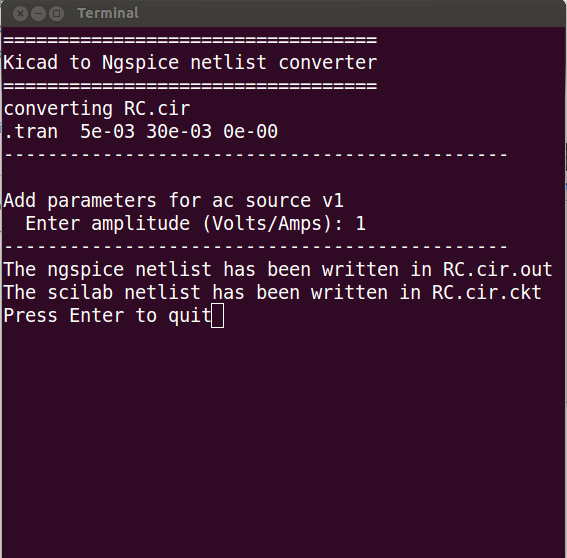
\includegraphics[width=\textwidth]{figures/16}
\caption{AC analysis example}
\label{16}
\end{figure}
Now we click on Kicad to Ngpice which will show the following terminal where we add the amplitude of AC and press 'enter' key.

After this we click on Ngspice button which will show Ngspice terminal with waveform window as shown in following figure:

We click on “analysis inserter” and then select type of analysis as “Transient” following window will appear:

now we add the details like “start time”, “step time”, “stop time”
